\title{
\centering

\includegraphics[width=4cm,height=4cm,keepaspectratio]{du.jpg} \\ \ CSE - 4255 Data Mining and Warehousing Lab\\  \Large \textit{Comparison Between the Performance of K - Means and K - Medoids Algorithm in Clustering}\\}


\author{
        Saif Mahmud \\
        Roll: SH - 54\\
            \and
        M. Tanjid Hasan Tonmoy\\
        Roll: SH - 09\\
            \and
        \\\textbf{Submitted To:}\\ Dr. Chowdhury Farhan Ahmed \\
        Professor\\
        \\ \& \\ 
        Abu Ahmed Ferdaus\\
        Associate Professor\\ \\
        Department of Computer Science and Engineering\\
        University of Dhaka        
}
\date{\today}

\documentclass[12pt]{article}
\usepackage{graphicx}
\usepackage{cite}
\usepackage{url}
\usepackage{multirow}
\usepackage{longtable}
\usepackage{multirow}
%\usepackage[a4paper]{geometry}
\newcommand{\s}{\vspace{0.2cm}}
\usepackage{float}

\begin{document}


\maketitle
\thispagestyle{empty}
\clearpage
\newpage

\section{Problem Definition}
In this experiment, we have implemented K-Means and K-Medoids Algorithm for Clustering. We have evaluated cluster quality in terms of purity measure and included analysis for determining number of clusters using elbow method. Execution time for varied number of clusters for both algorithms have been compared.

\section{Dataset Description}
Since the task at hand is targeted towards unsupervised segmentation of data, the datasets that have been selected do not have any class label annotations. We chose 3 datasets which we describe in the following subsections-

\subsection{Credit Card Unsupervised}
\label{credit}
The credit card dataset contains the usage record of 9000 credit card users over a period of 6 months. This data is available at kaggle.com\footnote{\url{https://www.kaggle.com/arjunbhasin2013/ccdata}} and contains 18 variables related to the particular customers behavior relating to finance. The attributes include account balance, frequency of balance updates, amount of purchases made from account etc. These categorical attributes do not include any class labels.

This data may be used to segment the customers into different groups so that a company may design effective marketing and advertising strategy. Such strategies may help to provide customized services and aid internal decision making.

\subsection{Weather Madrid 1997 - 2015}
This dataset\footnote{\url{https://www.kaggle.com/juliansimon/weather_madrid_lemd_1997_2015.csv}} contains the daily weather records of the city of Madrid from 1997 to 2015. There are 23 attributes in the that contains information such as minimum and maximum temperature, dew point, humidity etc. We exclude one column containing major weather event since majority of the data are missing.

Such dataset may help segment the days into different categories which may correspond to the seasons for example summer and winter days or more granular like hot and humid etc days depending on the number of clusters.

\subsection{Google Review Ratings}
This dataset includes reviews of different types of places from a number of visitors. Available in the UCI repository, this dataset may also help segment the visitors into groups similar to credit card dataset in subsection~\ref{credit}. The attributes contain ratings for different type of places.

\subsection{BuddyMove Data Set}
Containing user interest information extracted from user reviews published in the website holidayiq.com, this data may also be used for user segmentation similar to the google review dataset. The attributes contain the number of reviews a user has posted about some particular place type e.g.  theatres or parks.

\subsection{Summary}
\begin{table}[h]
	\label{tab:data}
	\caption{Dataset Statistics}
	\centering
	\begin{tabular}{|c|c|c|}
		\hline
		\textbf{Dataset} & \textbf{\begin{tabular}[c]{@{}c@{}}Number \\ of Samples\end{tabular}} & \textbf{\begin{tabular}[c]{@{}c@{}}Number \\ of Attributes\end{tabular}} \\ \hline
		Credit Card Unsupervised         & 8950                                                                            & 18 \\ \hline
		Weather Madrid 1997 - 2015            & 6812                                                                            & 23 \\ \hline
		Google Review Ratings           & 5456                                                                       & 24\\ \hline
		BuddyMove Data Set           & 250                                                                           & 6\\ \hline
	\end{tabular}
\end{table}


\section{Theory and Implementation}
\subsection{K - Means}
K - Means is centroid-based partitioning algorithm where the centroid of a cluster, represented by $C_i$ is used to represent the respective cluster.

\subsection{K - Medoids}
K-Medoids algorithm uses actual object from the data as representative for the clusters. Compared K-Means, this approach makes K-Medoids less sensitive to outliers. Each remaining object in the dataset is assigned to the cluster of the closest representative object.

K-medoids algorithm groups n objects into k clusters by minimizing the absolute error defined in (\ref{eq:km})

\begin{equation}
\label{eq:km}
 \sum_{i=1}^{k}\sum_{p \epsilon C_i} dist(p,o_i)
\end{equation}

The Partitioning Around Medoids (PAM) is an iterative, greedy
algorithm to implement k medoids since finding exact median every time incurs quadratic cost. Similar to k-means algorithm, the initial representative objects are randomly
chosen. It is considered whether replacing a representative object by a nonrepresentative
 would improve the clustering quality. All the possible replacements
are tried out. This process continues until the quality of the resulting clustering cannot be improved by performing any replacement. In our implementation,  a sampling-based method called CLARA (Clustering LARge Applications) has been used to deal with larger data sets. Instead of taking the whole data set into consideration, CLARA uses a random sample of the data set.

\section{Evaluation of Clustering}

\subsection{Elbow Method}

\begin{figure}[H]
	\centering
	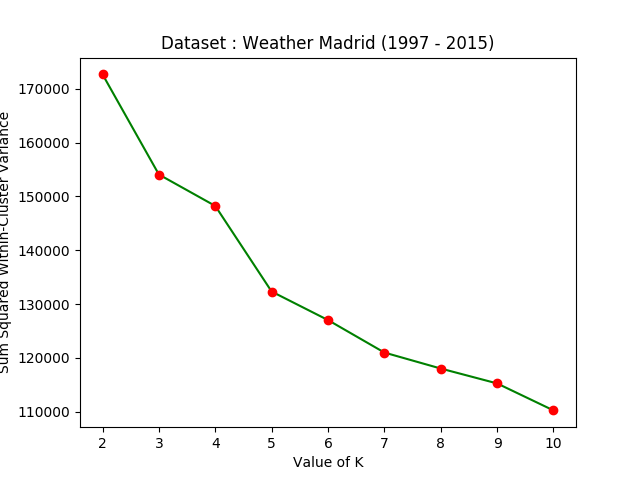
\includegraphics[width = \linewidth, height = 10.5cm]{Elbow_Weather.png}
	\caption{Determining Value of K through Elbow Method (K - Means)}
	\label{fig:elbow_weather}
\end{figure}

\begin{figure}[H]
	\centering
	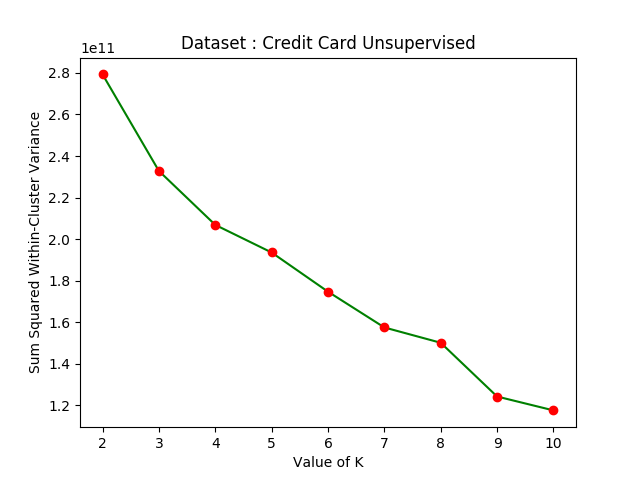
\includegraphics[width = \linewidth, height = 10.5cm]{Elbow_CreditCard.png}
	\caption{Determining Value of K through Elbow Method (K - Means)}
	\label{fig:elbow_credit}
\end{figure}

\subsection{Time Complexity Comparison}

\begin{figure}[H]
	\centering
	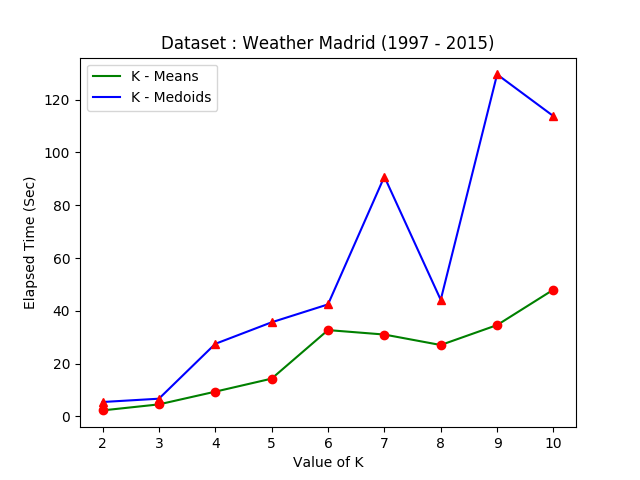
\includegraphics[width = \linewidth, height = 10.5cm]{Weather.png}
	\caption{Comparison of Elapsed Time between K - Means and K - Medoids Algorithm}
	\label{fig:weather}
\end{figure}

\begin{figure}[H]
	\centering
	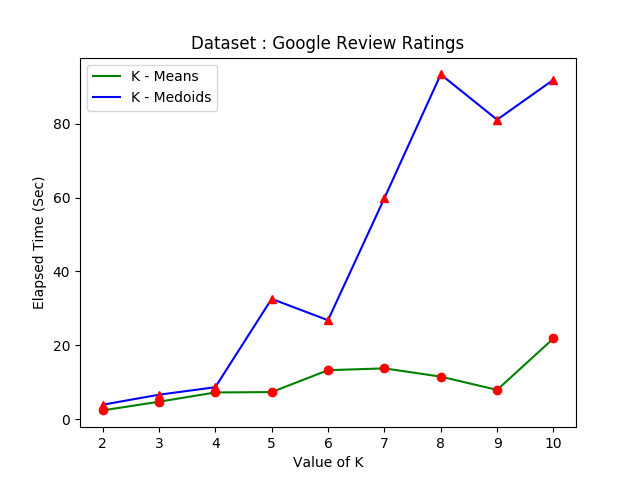
\includegraphics[width = \linewidth, height = 10.5cm]{Google.png}
	\caption{Comparison of Elapsed Time between K - Means and K - Medoids Algorithm}
	\label{fig:google}
\end{figure}

\begin{figure}[H]
	\centering
	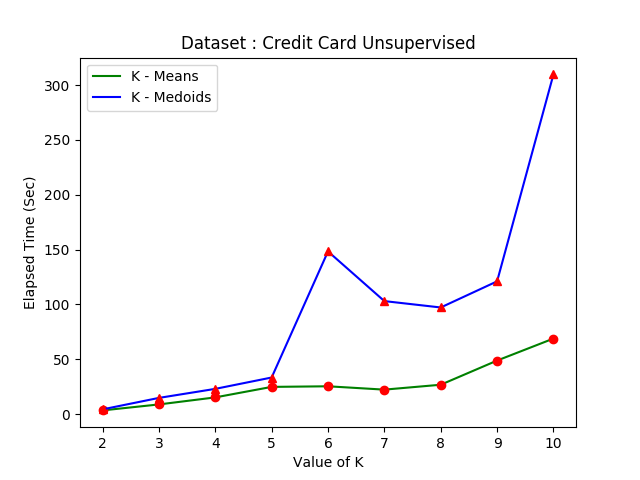
\includegraphics[width = \linewidth, height = 10.5cm]{CreditCard.png}
	\caption{Comparison of Elapsed Time between K - Means and K - Medoids Algorithm}
	\label{fig:credit}
\end{figure}



\section{Conclusion}



\end{document}
